% DO NOT COMPILE THIS FILE DIRECTLY!
% This is included by the other .tex files.

\begin{frame}[t,plain]
\titlepage
\end{frame}

\begin{frame}
\frametitle{What is Cerebrate?}
    \begin{itemize}
        \item A new-ish OSS Community management and orchestration platform
        \item Takes care of:
        \begin{itemize}
            \item {\bf Contact library} management
            \item {\bf Constituency} lookup
            \item {\bf Interconnection} Orchestration
            \item {\bf Tool management and orchestration}
            \item {\bf Sharing group} distribution and management
            \item {\bf Cryptographic key} lookup
            \item Shared services {\bf access management}
        \end{itemize}
        \item Developed initially as part of:
    \end{itemize}
    \vspace{0.5em}
    \begin{center}
        
\includegraphics[width=0.55\linewidth]{pictures/melicertes.png}
    \end{center}
\end{frame}

\begin{frame}
\frametitle{Managing large communities is difficult}
    \begin{itemize}
        \item Our MISP communities started out small
        \item Most communities acted as islands
        \item Interconnecting communities came with its own problems
        \begin{itemize}
            \item {\bf Interconnection requests}
            \item {\bf Organisation management}
            \item {\bf Enrollment} process
        \end{itemize}
        \item Finding and communicating with the right parties is difficult
        \item Managing multiple MISP instances can be tedious
    \end{itemize}
\end{frame}

\begin{frame}
\frametitle{A bit about our internal topology}
  \begin{center}
    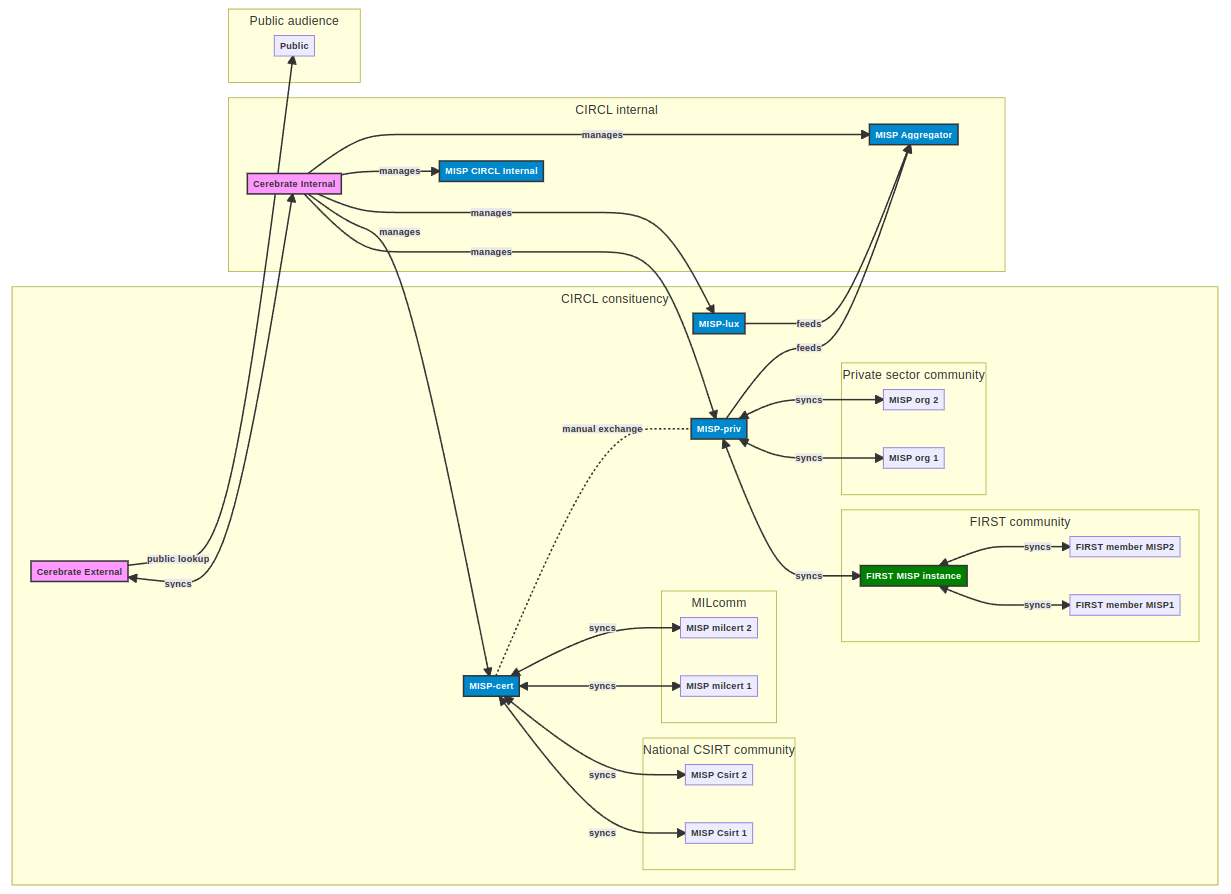
\includegraphics[width=1\linewidth]{pictures/our_topology.png}
  \end{center}
\end{frame}

\begin{frame}
    \frametitle{Some stats about one of our MISP instance: MISPPriv}
      \begin{center}
    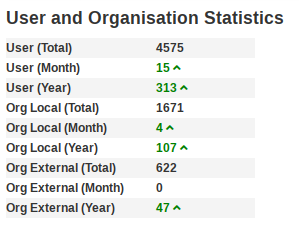
\includegraphics[width=0.6\linewidth]{pictures/misppriv-user-org-stats.png}
      \end{center}
\end{frame}

\begin{frame}
\frametitle{Issues we're trying to solve}
    \begin{itemize}
        \item {\bf Contact management} across large interconnected networks
        \begin{itemize}
            \item ORG uuids, capabilities, individuals, etc
        \end{itemize}
        \item {\bf Constituency} information
         \begin{itemize}
            \item Geographic \& sectorial
            \item But also technical: CIDR blocks \& AS Numbers
        \end{itemize}
	\item Managing local tools, especially {\bf fleets of MISPs}
	\item Common access control management
	\item {\bf Distribution list} management
	\item MISP cryptographic signing {\bf PKI} management
	 \begin{itemize}
            \item MISP's protected event feature
            \item Future: Protected Sharing groups? 
        \end{itemize}
        \item Community centric {\bf data modelling}
    \end{itemize}
\end{frame}

\begin{frame}
\frametitle{Cerebrate's contact database}
    \begin{itemize}
        \item Contact database for the CSIRT network
        \begin{itemize}
            \item Common contact fields such as \texttt{UUID}, \texttt{name}, \texttt{contact email address}, \texttt{nationality}, \texttt{URL}, ...
        \end{itemize}
    \end{itemize}
    \begin{center}
        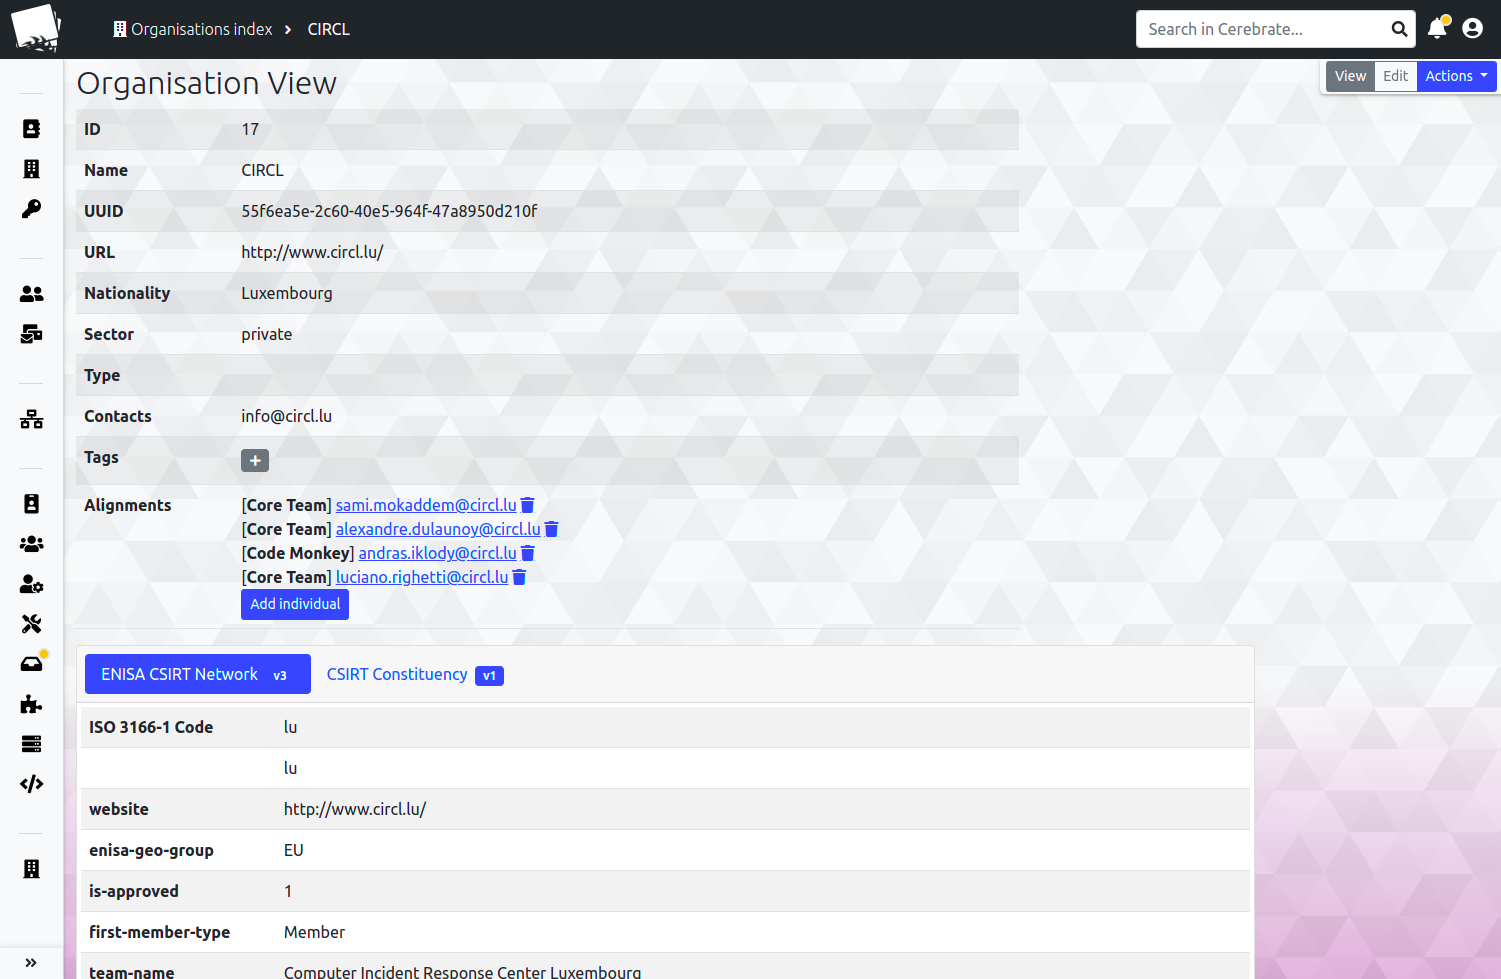
\includegraphics[width=0.8\linewidth]{pictures/contact-database-1.png}
    \end{center}
\end{frame}

\begin{frame}
\frametitle{Cerebrate's contact database: Meta-fields}
    \begin{itemize}
        \item Flexible system to store additional information: \texttt{meta-fields} (KV-store)
        \item These \texttt{meta-fields} are part of a larger structure called \texttt{meta-templates}
        \item Support of {\bf multiple templates} used by various entities out there
        \begin{itemize}
            \item FIRST Directory
            \item ENISA CSIRT inventory
            \item CSIRT Constituency (CIDR blocks, AS Numbers, ...)
        \end{itemize}
    \end{itemize}
\end{frame}

\begin{frame}
\frametitle{Cerebrate's contact database: Meta-fields}
\begin{center}
    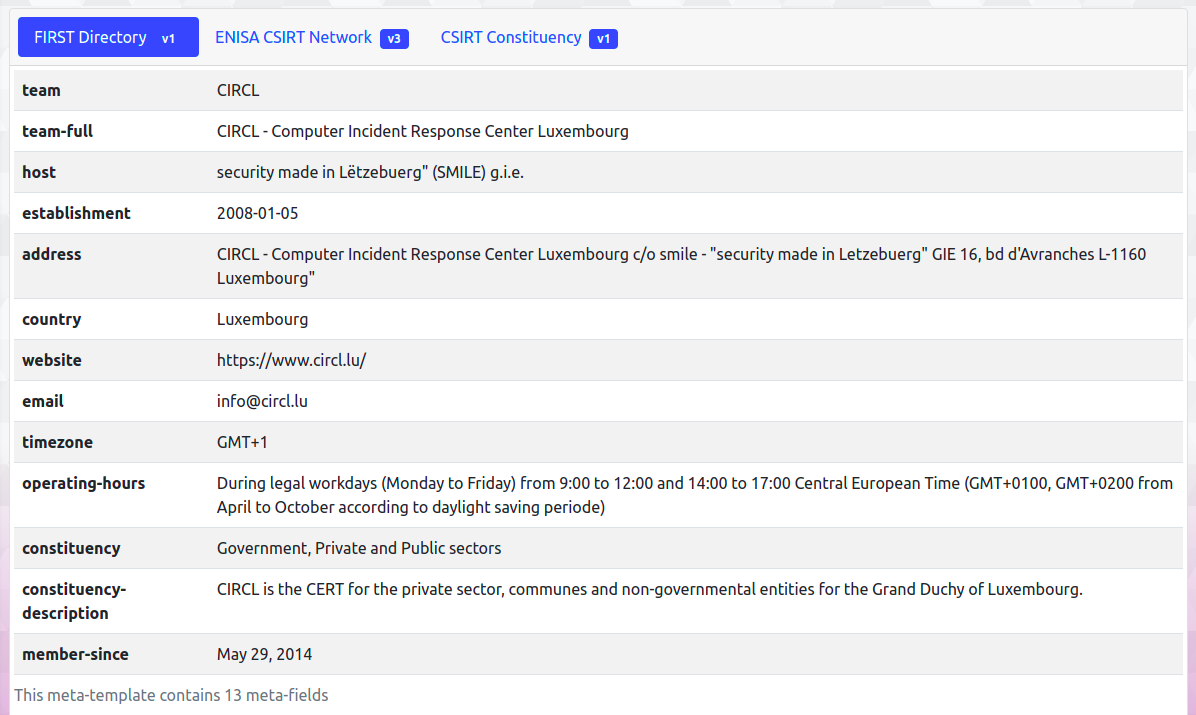
\includegraphics[width=0.99\linewidth]{pictures/meta-fields-first.png}
\end{center}
\end{frame}


\begin{frame}
\frametitle{Cerebrate's contact database}
    \begin{center}
        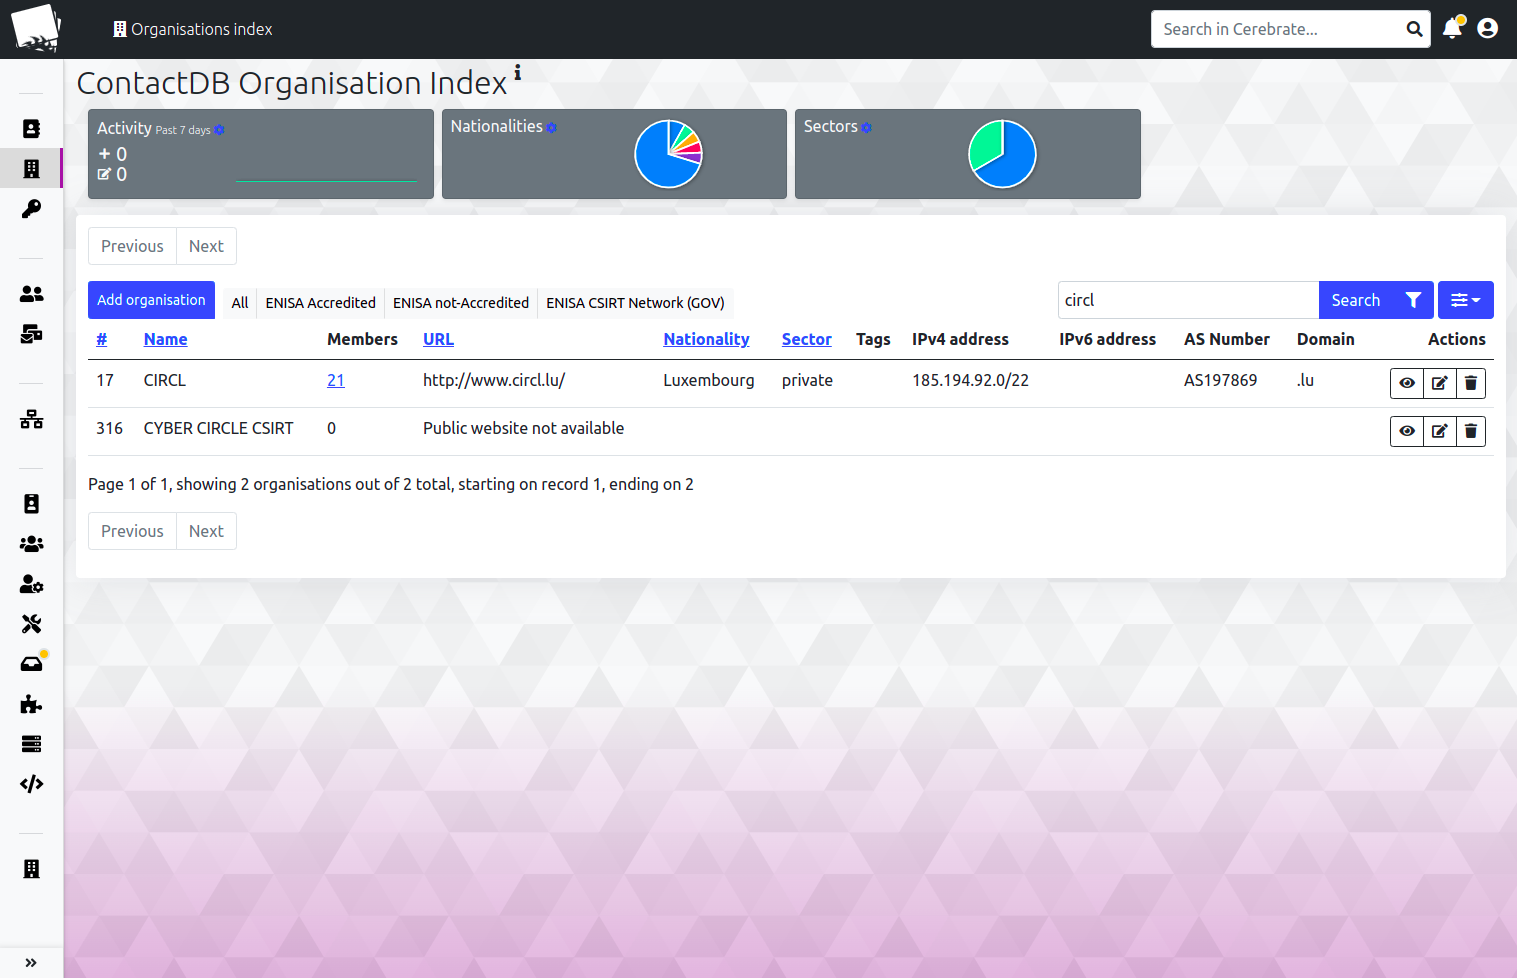
\includegraphics[width=0.99\linewidth]{pictures/contact-database-2.png}
    \end{center}
\end{frame}



\begin{frame}
\frametitle{Managing local tools}
    \begin{itemize}
        \item Cerebrate exposes a modular system to {\bf manage these local tools}
        \item Based on a configuration file, user interfaces can be created to visualise data and instruct local tools to perform operations
    \end{itemize}
    \begin{center}
        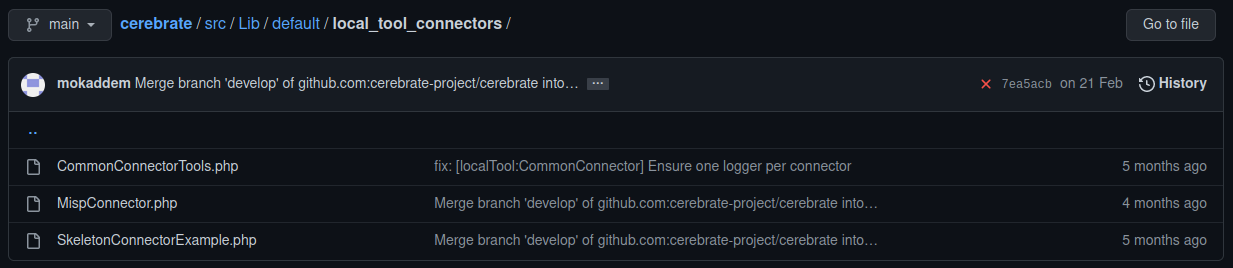
\includegraphics[width=1.0\linewidth]{pictures/github-local-tool.png}
    \end{center}
\end{frame}

\begin{frame}
\frametitle{Local tools: MISP Connector capabilities}
    \begin{itemize}
        \item \textbf{Configure} a MISP instances via server settings
        \item \textbf{Push and Pull} Organisations \& Sharing Groups
        \item \textbf{Diagnose} other connected MISP servers
        \item \textbf{Manage} users
        \item \textbf{Custom} actions are easy to integrated beyond the initial scope
    \end{itemize}
\end{frame}

\begin{frame}
\frametitle{Local tool interconnection via Cerebrate}
    \begin{itemize}
        \item Cerebrate's main goal is to \textbf{ease community management}
        \item Select which local tools are meant to be exposed to the community for requests
        \item Open dialogues to community members to request tool-to-tool interconnections
    \end{itemize}
\end{frame}

\begin{frame}
\frametitle{Local tool interconnection via Cerebrate}
    Cerebrate can leverage its access to local tool to reach out to tools from other Cerebrate nodes
    \begin{center}
        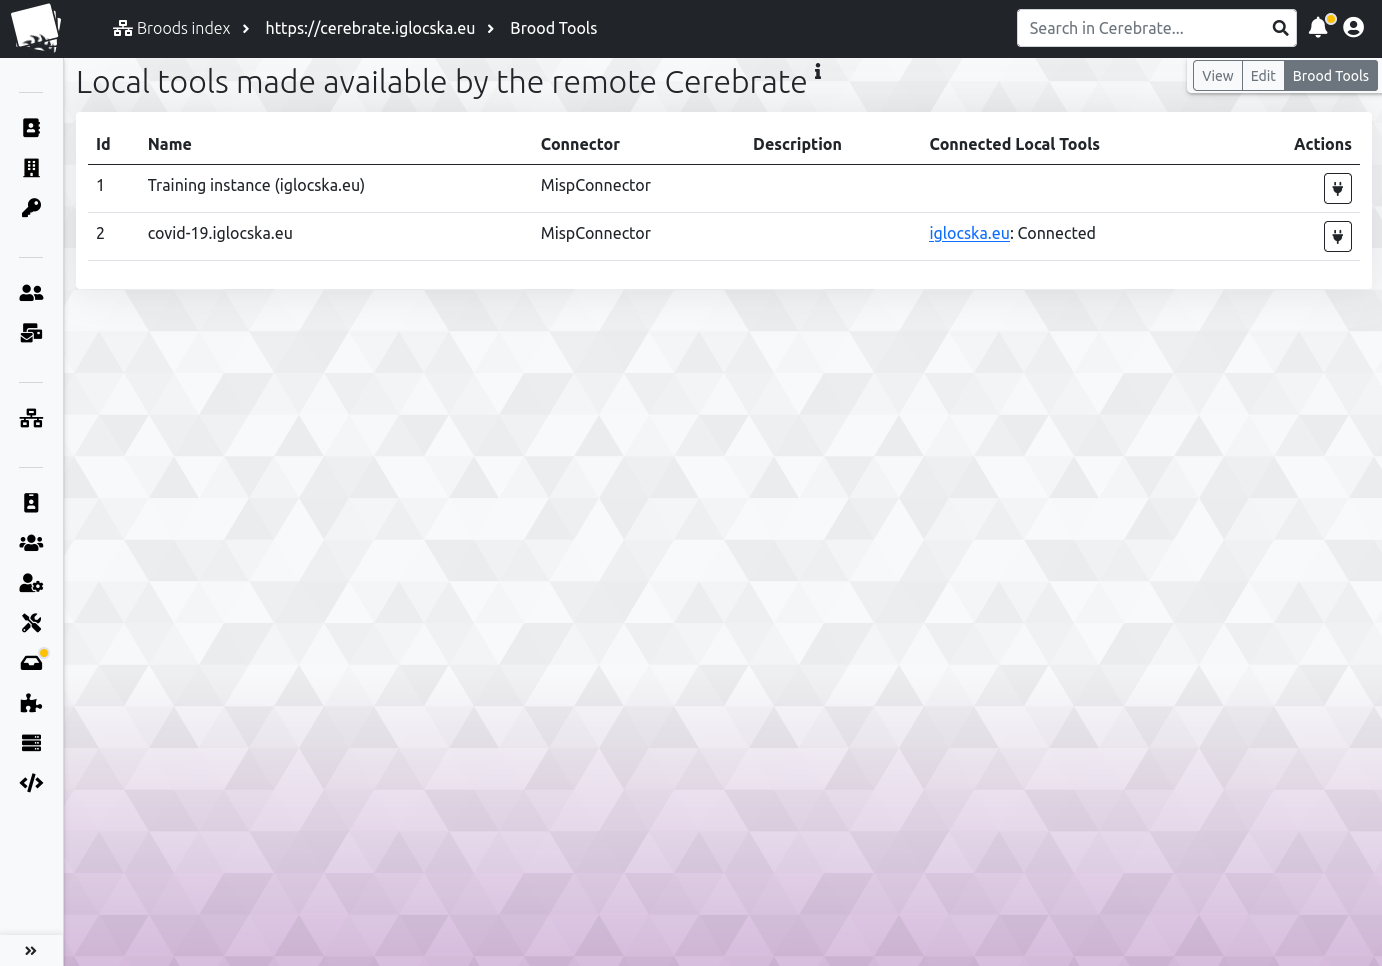
\includegraphics[width=0.85\linewidth]{pictures/tools-made-available.png}
    \end{center}
\end{frame}

\begin{frame}
\frametitle{Development update}
    \begin{itemize}
        \item 6 releases
        \item 388 commits
        \item Ongoing work on the community management aspect...
        \item ...as well as orchestration
    \end{itemize}
\end{frame}

\begin{frame}
\frametitle{Development update}
    \begin{itemize}
        \item A long list of fixes and improvements
        \item Tight collaboration with {\bf ENISA and the CSIRT-network}
        \item Ongoing pilot programme at CNW
        \item Implementing new CSIRT-network use-cases
    \end{itemize}
\end{frame}

\begin{frame}
\frametitle{Development update}
    \begin{itemize}
        \item Improved {\bf controls via customisable, IAM exposed permissions}
        \item Tooling for creating {\bf vocabularies for custom field pre-sets} (enumerations)
        \item Versioning and updates of existing data for new metafield library versions
        \item An additional layer of grouping and self-governance
    \end{itemize}
\end{frame}

\begin{frame}
\frametitle{Upcoming fleet release}
    \begin{itemize}
        \item New graphical UI for managing local tools and sync connections
        \item Rework of sharing groups to be closer in-line with MISP
        \item Diagnostic tools for MISP instances, exposing common misconfigurations
        \begin{itemize}
          \item PHP settings
          \item Worker health and stuck queues
          \item Out of date warnings
          \item MySQL settings
        \end{itemize}
        \item Improvements to the local tool common tools library
    \end{itemize}
\end{frame}

\begin{frame}
\frametitle{Fleet management}
  \begin{center}
    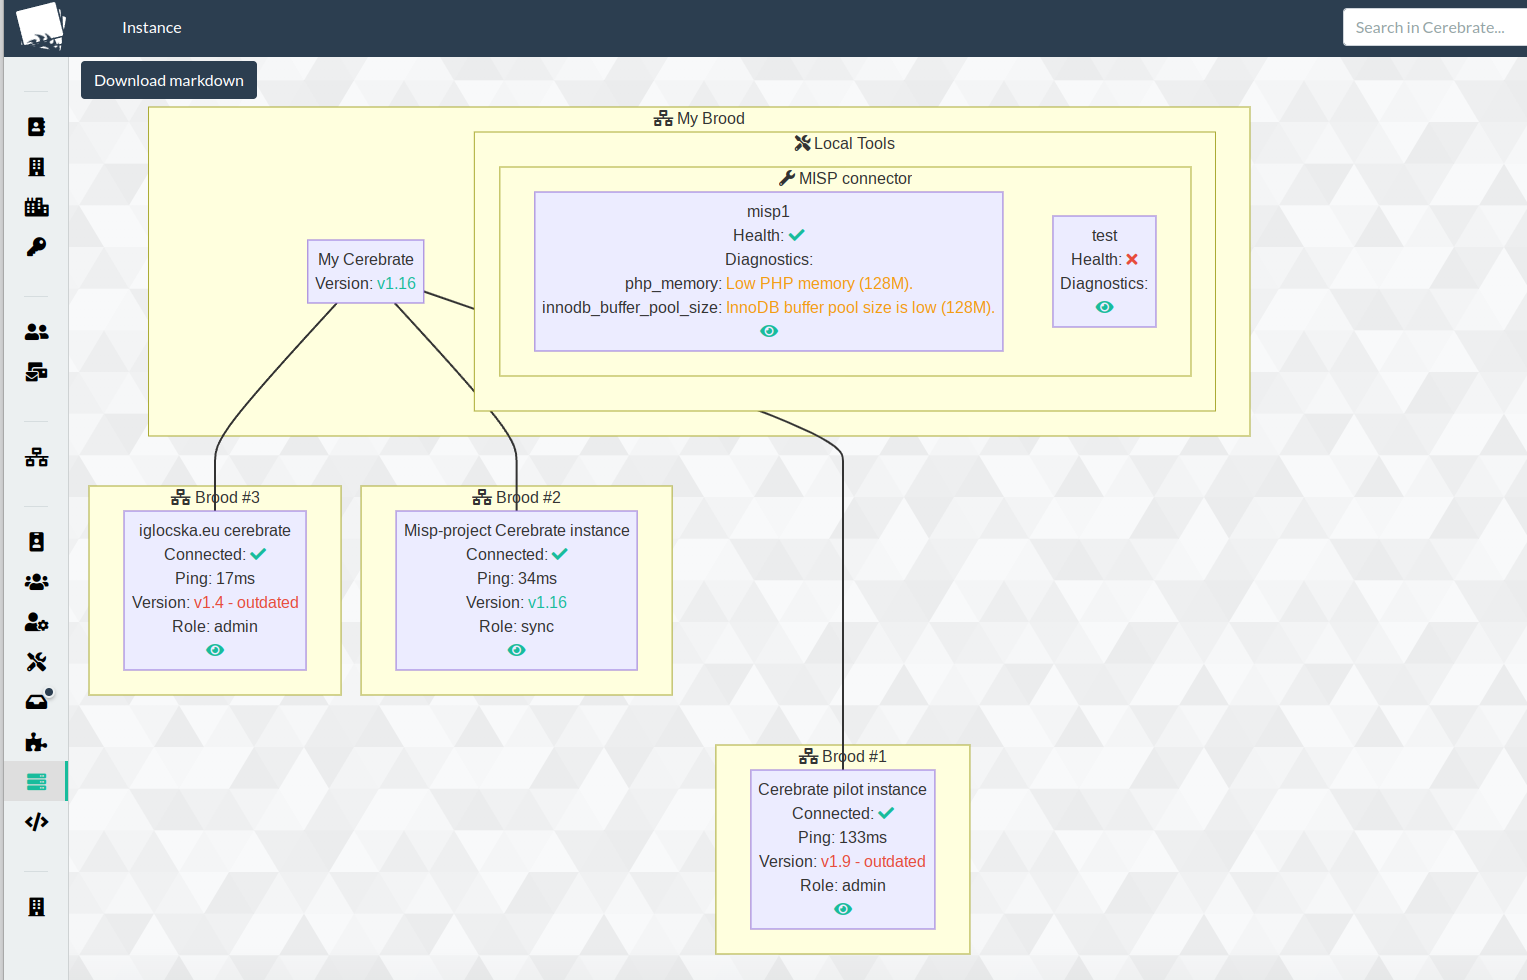
\includegraphics[width=1\linewidth]{pictures/topology.png}
  \end{center}
\end{frame}

\begin{frame}
\frametitle{Fleet management}
  \begin{center}
    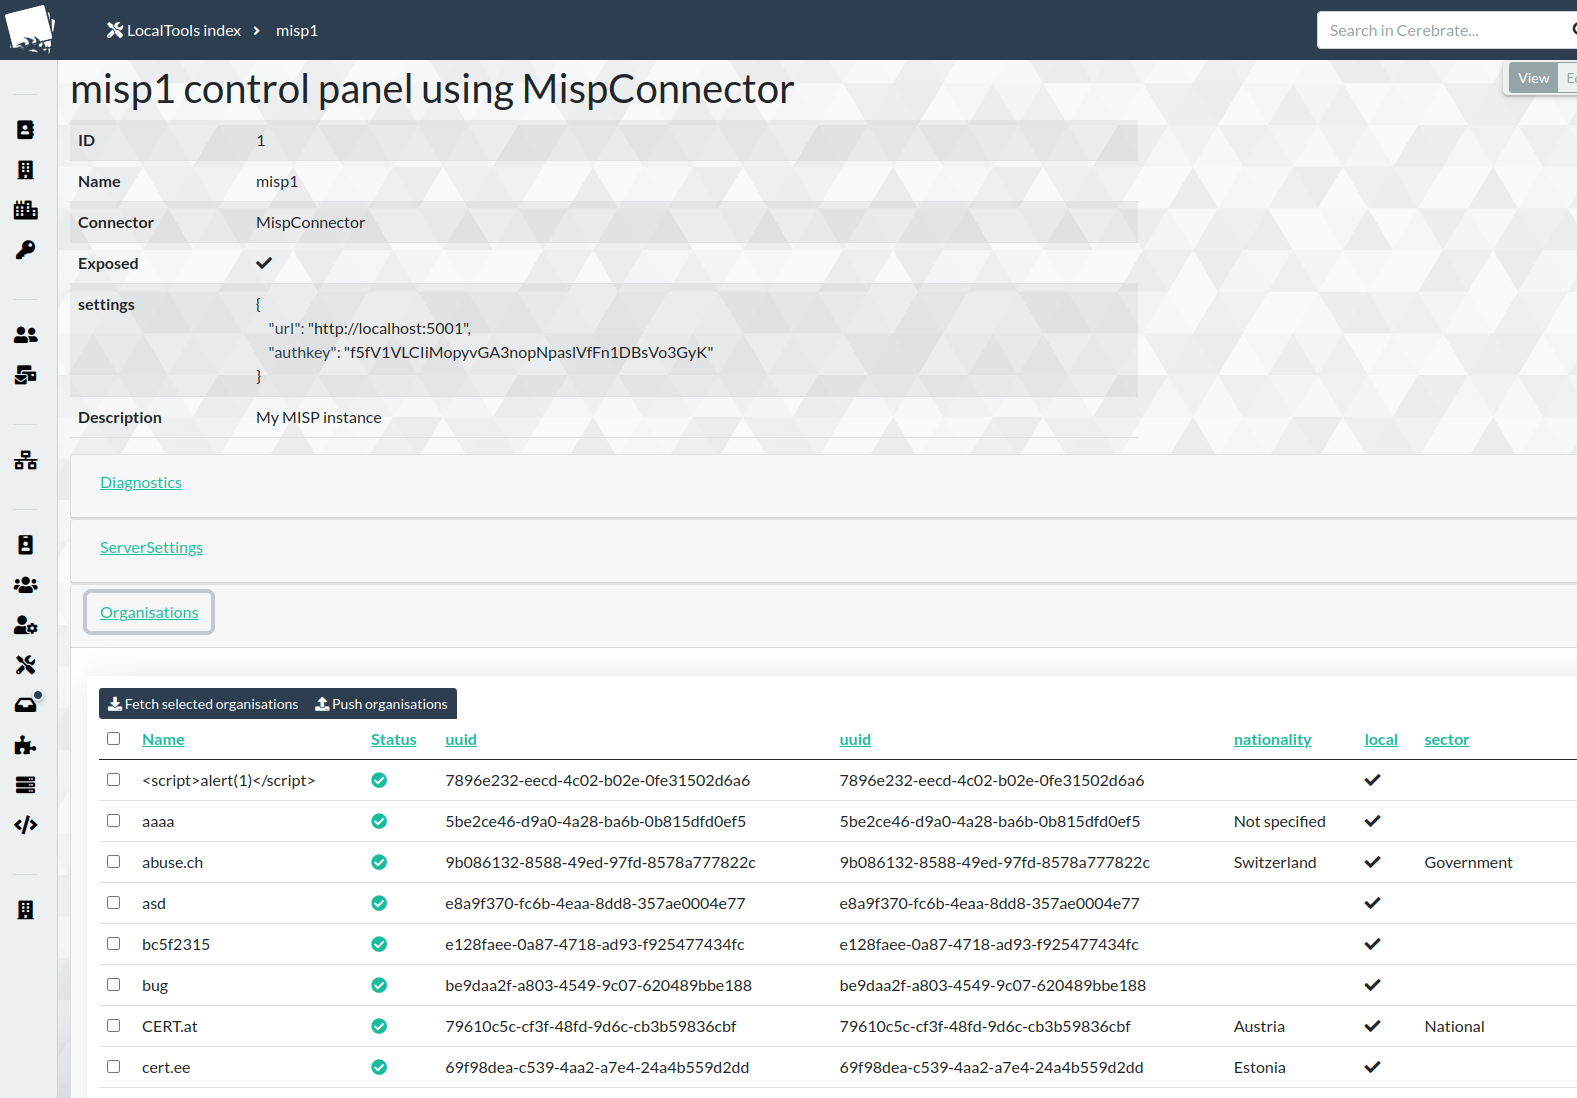
\includegraphics[width=1\linewidth]{pictures/fleet2.png}
  \end{center}
\end{frame}


\begin{frame}
\frametitle{Current roadmap}
    \begin{itemize}
        \item Upcoming {\bf fleet management} release
        \item {\bf Sharing groups} rework
        \item Data {\bf signing / validation}
        \begin{itemize}
            \item Community centric PKI
            \item Enable data validation services for tools such as MISP
        \end{itemize}
        \item {\bf Integration with other tools}
        \begin{itemize}
            \item Ticketing systems
            \item Tighter Mailing list integration (Mailman)
            \item Messaging App (Mattermost)
        \end{itemize}
    \end{itemize}
\end{frame}
